\documentclass{article} % say
\usepackage{tikz}
\usetikzlibrary{calc,arrows,fit,positioning}


\begin{document}

\centering
    
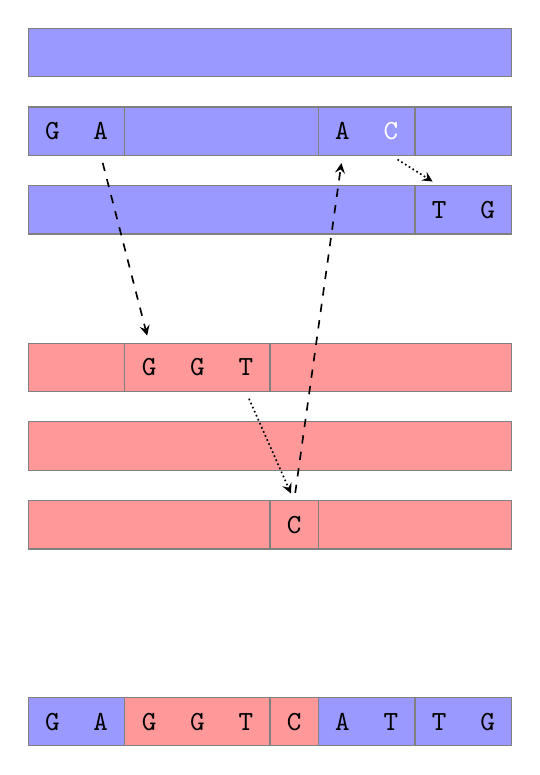
\begin{tikzpicture}[scale=0.5]

\tikzset{inner sep=0mm,minimum width=6mm,minimum height=6mm,
pop1/.style={fill=blue!40,draw=black!50},
pop2/.style={fill=red!40,draw=black!50},
hapjump/.style={->,>=stealth,semithick,shorten <=1mm,shorten >=1mm,semithick,densely dotted},
ancjump/.style={->,>=stealth,semithick,shorten <=1mm,shorten >=1mm,semithick,dashed}}

% Focal sequence
\node (h0) {$\texttt{G}$};
\node (h1) [right=0mm of h0,node distance=0mm] {$\texttt{A}$};
\node (h2) [right=0mm of h1] {$\texttt{G}$};
\node (h3) [right=0mm of h2] {$\texttt{G}$};
\node (h4) [right=0mm of h3] {$\texttt{T}$};
\node (h5) [right=0mm of h4] {$\texttt{C}$};
\node (h6) [right=0mm of h5] {$\texttt{A}$};
\node (h7) [right=0mm of h6] {$\texttt{T}$};
\node (h8) [right=0mm of h7] {$\texttt{T}$};
\node (h9) [right=0mm of h8] {$\texttt{G}$};
\node[draw=black,fit=(h0) (h9)] (chrom) {};


% Nodes: reference sequences
\node (ref1) at (0,5) {};
\node (ref2) at (0,13) {};
\node (sam1) at (0,0) {};
\node (sam2) at (0,2) {};
\node (sam3) at (0,4) {};

% Draw reference sequences

%pop2
\node (chr1A0) at ($(h0) + (ref1) + (sam1)$) {\textcolor{white}{$\texttt{C}$}};
\node (chr1A9) at ($(h9) + (ref1) + (sam1)$) {\textcolor{white}{$\texttt{C}$}};
\node[pop2,fit=(chr1A0) (chr1A9)] (chr1A) {};

\node (chr1B0) at ($(h0) + (ref1) + (sam2)$) {\textcolor{white}{$\texttt{C}$}};
\node (chr1B9) at ($(h9) + (ref1) + (sam2)$) {\textcolor{white}{$\texttt{C}$}};
\node[pop2,fit=(chr1B0) (chr1B9)] (chr1B) {};

\node (chr1C0) at ($(h0) + (ref1) + (sam3)$) {\textcolor{white}{$\texttt{C}$}};
\node (chr1C9) at ($(h9) + (ref1) + (sam3)$) {\textcolor{white}{$\texttt{C}$}};
\node[pop2,fit=(chr1C0) (chr1C9)] (chr1C) {};

\node (chr2A0) at ($(h0) + (ref2) + (sam1)$) {\textcolor{white}{$\texttt{C}$}};
\node (chr2A9) at ($(h9) + (ref2) + (sam1)$) {\textcolor{white}{$\texttt{C}$}};
\node[pop1,fit=(chr2A0) (chr2A9)] (chr2A) {};

\node (chr2B0) at ($(h0) + (ref2) + (sam2)$) {\textcolor{white}{$\texttt{C}$}};
\node (chr2B9) at ($(h9) + (ref2) + (sam2)$) {\textcolor{white}{$\texttt{C}$}};
\node[pop1,fit=(chr2B0) (chr2B9)] (chr2B) {};

\node (chr2C0) at ($(h0) + (ref2) + (sam3)$) {\textcolor{white}{$\texttt{C}$}};
\node (chr2C9) at ($(h9) + (ref2) + (sam3)$) {\textcolor{white}{$\texttt{C}$}};
\node[pop1,fit=(chr2C0) (chr2C9)] (chr2C) {};



%%%%%%%%%%%%%%

% Chunks on focal sequence
\node[pop1,fit=(h0) (h1)] (chunk1) {};
\node[pop2,fit=(h2) (h4)] (chunk2) {};
\node[pop2,fit=(h5) (h5)] (chunk3) {};
\node[pop1,fit=(h6) (h7)] (chunk4) {};
\node[pop1,fit=(h8) (h9)] (chunk5) {};


\node (h0) {$\texttt{G}$};
\node (h1) [right=0mm of h0,node distance=0mm] {$\texttt{A}$};
\node (h2) [right=0mm of h1] {$\texttt{G}$};
\node (h3) [right=0mm of h2] {$\texttt{G}$};
\node (h4) [right=0mm of h3] {$\texttt{T}$};
\node (h5) [right=0mm of h4] {$\texttt{C}$};
\node (h6) [right=0mm of h5] {$\texttt{A}$};
\node (h7) [right=0mm of h6] {$\texttt{T}$};
\node (h8) [right=0mm of h7] {$\texttt{T}$};
\node (h9) [right=0mm of h8] {$\texttt{G}$};


% Chunks from reference sequences


%pop2

\node (chr1A5) at ($(h5) + (ref1) + (sam1)$) {};
\node[pop2,fit=(chr1A5) (chr1A5)] (chunk1A) {};
\node (chr1A5) at ($(h5) + (ref1) + (sam1)$) {$\texttt{C}$};

\node (chr1C2) at ($(h2) + (ref1) + (sam3)$) {};
\node (chr1C3) at ($(h3) + (ref1) + (sam3)$) {};
\node (chr1C4) at ($(h4) + (ref1) + (sam3)$) {};
\node[pop2,fit=(chr1C2) (chr1C4)] (chunk1C) {};
\node (chr1C2) at ($(h2) + (ref1) + (sam3)$) {$\texttt{G}$};
\node (chr1C3) at ($(h3) + (ref1) + (sam3)$) {$\texttt{G}$};
\node (chr1C4) at ($(h4) + (ref1) + (sam3)$) {$\texttt{T}$};


%pop1
\node (chr2A8) at ($(h8) + (ref2) + (sam1)$) {};
\node (chr2A9) at ($(h9) + (ref2) + (sam1)$) {};
\node[pop1,fit=(chr2A8) (chr2A9)] (chunk2A) {};
\node (chr2A8) at ($(h8) + (ref2) + (sam1)$) {$\texttt{T}$};
\node (chr2A9) at ($(h9) + (ref2) + (sam1)$) {$\texttt{G}$};

\node (chr2B0) at ($(h0) + (ref2) + (sam2)$) {};
\node (chr2B1) at ($(h1) + (ref2) + (sam2)$) {};
\node (chr2B6) at ($(h6) + (ref2) + (sam2)$) {};
\node (chr2B7) at ($(h7) + (ref2) + (sam2)$) {};
\node[pop1,fit=(chr2B0) (chr2B1)] (chunk2B1) {};
\node[pop1,fit=(chr2B6) (chr2B7)] (chunk2B2) {};
\node (chr2B0) at ($(h0) + (ref2) + (sam2)$) {$\texttt{G}$};
\node (chr2B1) at ($(h1) + (ref2) + (sam2)$) {$\texttt{A}$};
\node (chr2B6) at ($(h6) + (ref2) + (sam2)$) {$\texttt{A}$};
\node (chr2B7) at ($(h7) + (ref2) + (sam2)$) {\textcolor{white}{$\texttt{C}$}};

% Arrows
\draw[ancjump] (chr2B1.south) -- (chr1C2.north);
%\node (leave chr2B1) [below=of chr2B1]) edge [ancjump] (chr1C2);


\draw[hapjump] (chr1C4.south) -- (chr1A5.north);
\draw[ancjump] (chr1A5.north) -- (chr2B6.south);
\draw[hapjump] (chr2B7.south) -- (chr2A8.north);



\end{tikzpicture}  

\end{document}